\section{3G og GPS shield til arduino}

\subsection{3G modul}
For at kunne kommunikere mellem webapplikation og drone er det nødvendigt at dronen har forbindelse til internettet. 
Der kræves en hurtig og stabil internetforbindelse, da dronen under flyvning både skal sende billeder og modtage kommandoer fra webapplikation.

Til at kunne sende informationer mellem webapplikation og dronen er det besluttet at anvende GPRS protokollen eller højere. Idet der skal sendes billeder fra dronen og til webapplikationen, kræver det en stabil og hurtig forbindelse, for at reducere tiden dronen skal bruge på at vente på godkendelse.

Nedenunder er et billede der viser de forskellige hastigheder fra 3G protokollen og nedefter. 

\begin{figure}[H]
\centering
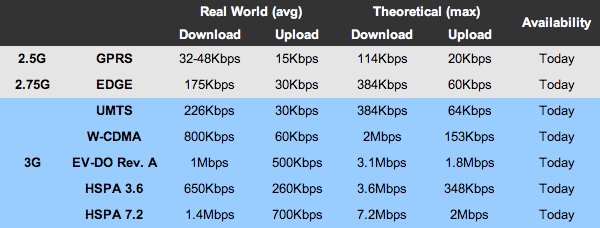
\includegraphics[width=0.7\textwidth]{Billeder/3g-table.png}
\caption[trådløs_teknologi]{trådløs teknologi\protect\footnotemark}
\label{fig:3gtable}
\end{figure}
\footnotetext{http://www.techspot.com/guides/272-everything-about-4g/}


Valg af 3G modul er foretaget på følgende kriterier:

\begin{itemize}
	\item Overføringshastighed.
	\item Pris.
	\item Kompatibel med arduino.
\end{itemize}

Ved at følge kriterierne, har vi fundet frem til følgende moduler der kan anvendes:

Sparkfuns\footnote{https://www.sparkfun.com/products/9607} Cellular Shield. \newline 
Dette shield kan bruges sammen med en arduino, hvor det fungerer som et shield der skal placeres på arduinoen.
Dog understøtter dette shield kun GPRS og nedefter. Som vist på Figur~\ref{fig:3gtable} kan GPRS kun uploade optil 20 Kbps teoretisk og $\sim$15 Kbps og for virkeligheden.

Cooking-Hacks har lavet et shield\footnote{http://www.cooking-hacks.com/documentation/tutorials/arduino-3g-gprs-gsm-gps}. Dette shield understøtter brugen af 3G, hvilket giver den en upload hastighed optil $\sim$2Mbps teoretisk og $\sim$700Kbps for virkeligheden, se Figur~\ref{fig:3gtable}.

Begge shields har mulighed for at transmittere data mellem dronen og webapplikationen. Cookings Hacks' 3G shield er dog en bedre løsning. Da det understøtter et nyere mobilt netværk, der giver mulighed for at sende og modtage data med større datarater.
Ved sammenligning af prisen ses det, at Cooking Hacks shieldet koster mere end Sparkfuns, dog har Cooking Hacks shieldet den fordel at den udover 3G også indeholder GPS.

\subsection{GPS}

På grund af Cooking Hacks' 3G modul med indbygget GPS, blev valget automatisk truffet. 
3G-GPS shieldet har mulighed for forskellige modes: \textit{mobile-assisted, mobile-based \& standalone}. De forskellige modes gør det muligt at bruge GPS sammen med eller uden netværk. \newline 
Hvis GPS'en anvendes sammen med netværk, bliver GPS koordinaterne bearbejdet og sendt til den ønskede enhed, mens den i \textit{standalone} giver koordinaerne direkte fra satellitterne.

